\documentclass[../../main.tex]{subfiles}

\begin{document}

    Zu Beginn unserer Messung stehen bereits vorausgewählte Parameter zur Messung des FID. Diese sind in Abbildung \ref{fig:2:Parameter} aufgetragen. Durch Fouriertransformation erhalten wir im Frequenzraum ein zum FID zugehöriges Spektrum, wie in Abbildung \ref{fig:2:Spectrum} abgebildet. Das FID Signal ist bereit zu Versuchsbeginn in deutlicher Form zu erkennen und weist keine nennenswerten Störungen auf, wie in Abbildung \ref{fig:2:FID12} zu sehen ist. Die Larmorfrequenz $f_L$ ist dabei durch die Frequenz des Peaks im Spektrum gegeben, also als funktionsmaximierendes Argument. Dieses bestimmen wir durch direkte Datensatzanalyse. Diesen Datensatz generieren wir mithilfe der Computersoftware Prospa und dem Messmodus \enquote{Pulse and Collect}. 
    \begin{figure}[H]
        \centering
        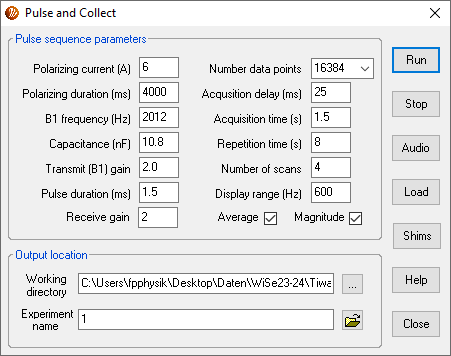
\includegraphics[width=8cm]{Bilddateien/2/Exp1_Parameter.PNG}
        \caption{Vorausgewählte Parameter zur Messung des FID.}
        \label{fig:2:Parameter}
    \end{figure}
    Als erste Ergebnisse erhalten wir die direkten Messungen der FIDs in zwei von uns durchgeführten aufeinanderfolgenden Durchgängen.
    \begin{figure}[H]
        \centering
        \begin{subfigure}[b]{0.4\textwidth}
            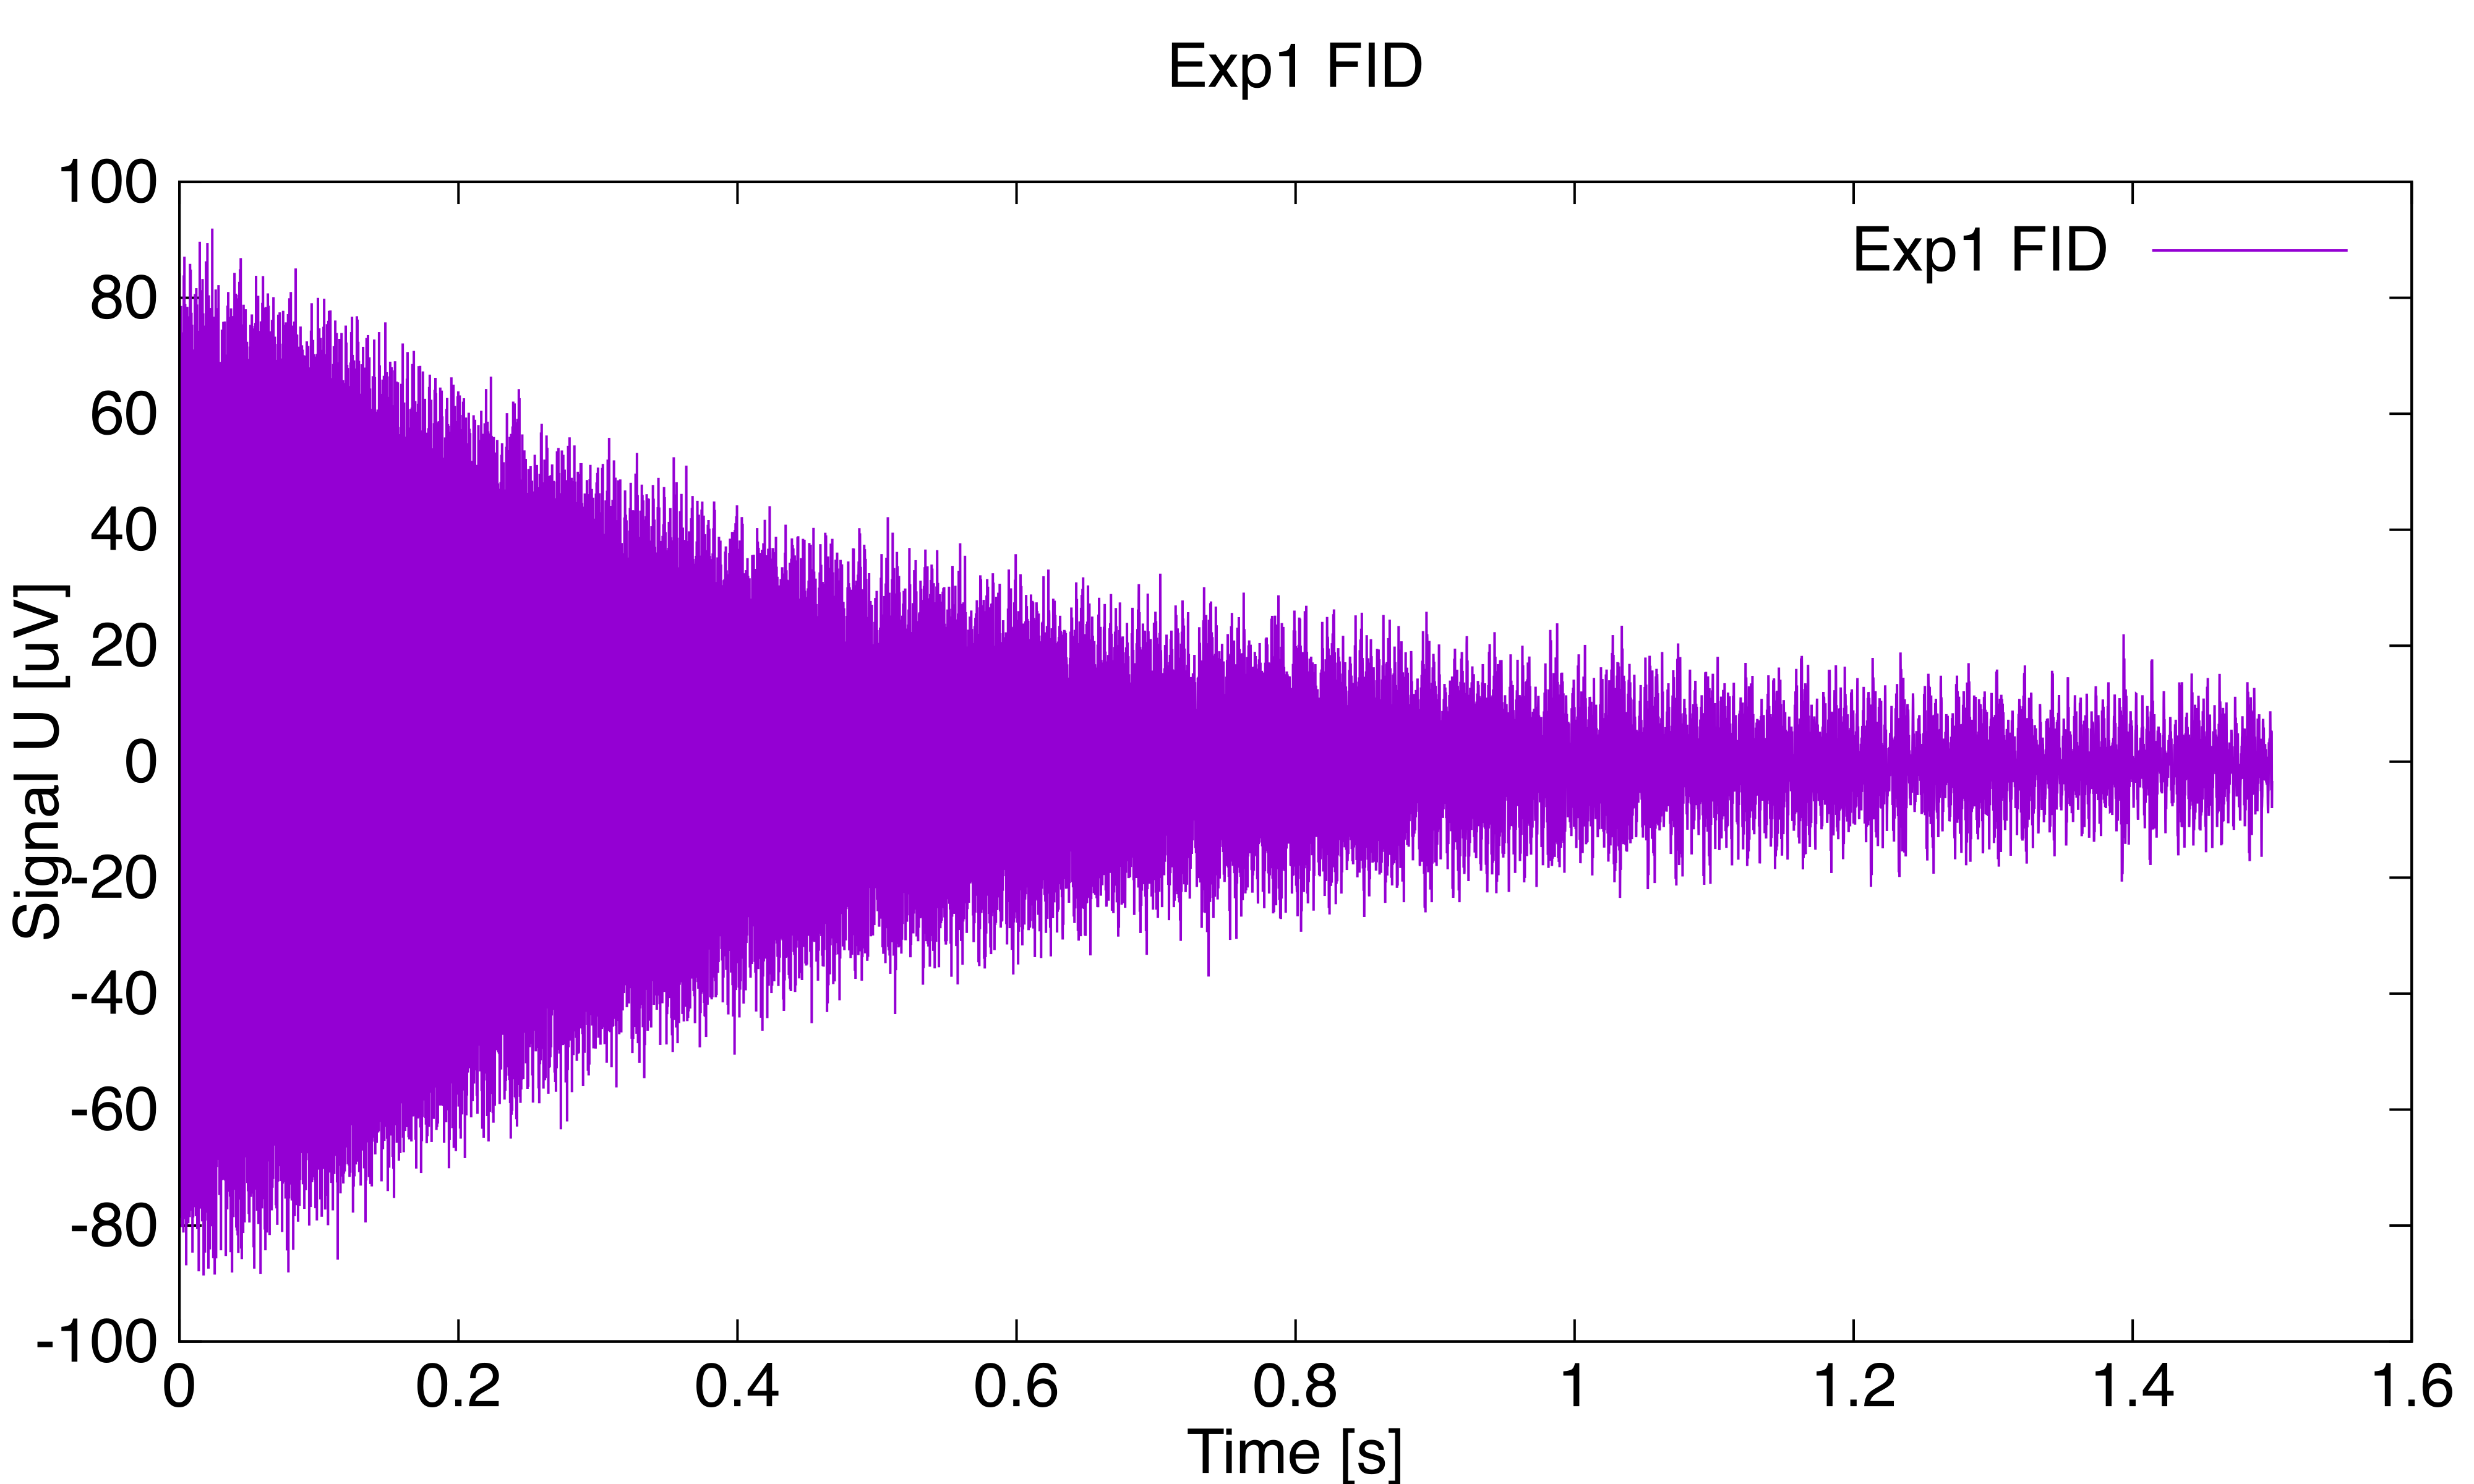
\includegraphics[width=6cm]{Bilddateien/2/Exp1_FID.png}
            \caption{FID Signal des ersten Durchgangs.}
            \label{fig:2:FID1}
        \end{subfigure}
        \
        \begin{subfigure}[b]{0.4\textwidth}
            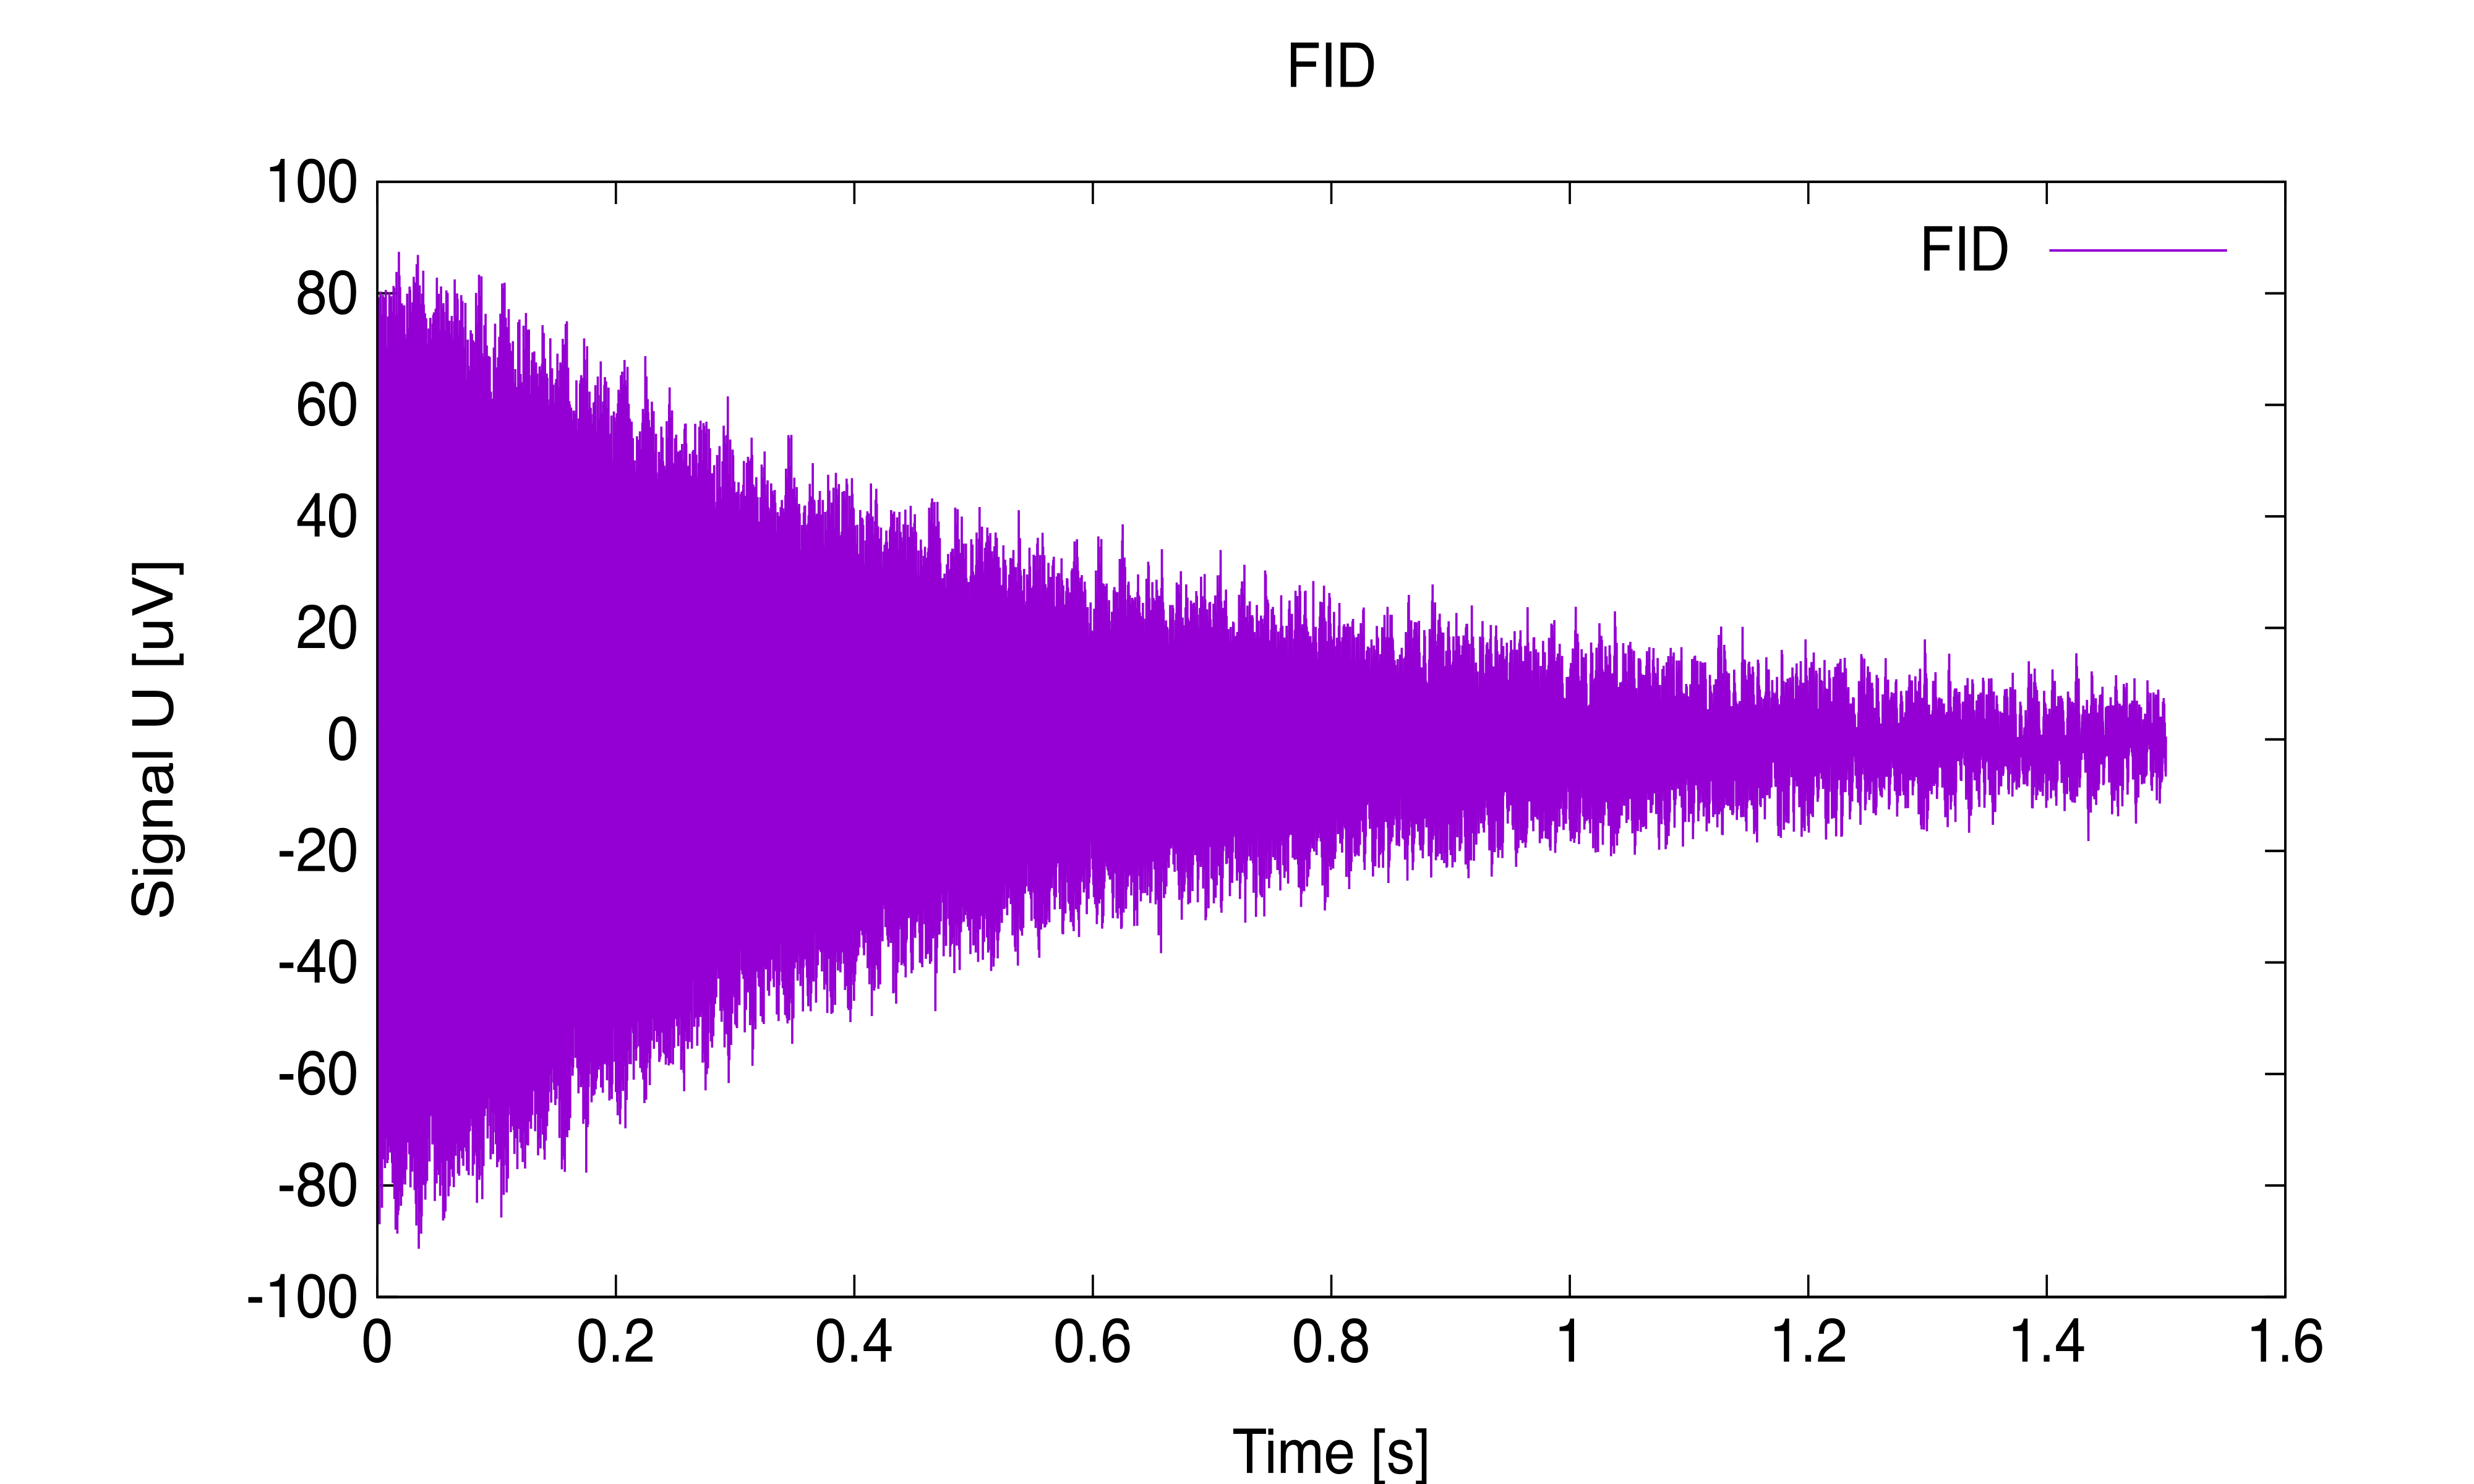
\includegraphics[width=6cm]{Bilddateien/2/Exp2_FID.png}
            \caption{FID Signal des zweiten Durchgangs.}
            \label{fig:2:FID2}
        \end{subfigure}
        \caption{FID Signal und Spektrum des FIDs.}
        \label{fig:2:FID12}
    \end{figure}
    Durch bereits in die Software integrierte Fouriertransformation erhalten wir die Spektren der FIDs, wie in Abbildung \ref{fig:2:Spectrum} zu sehen ist. Die Larmorfrequenz $f_L$ lässt sich hier bereits mit dem Auge erahnen.
    \begin{figure}[H]
        \centering
        \begin{subfigure}[b]{0.4\textwidth}
            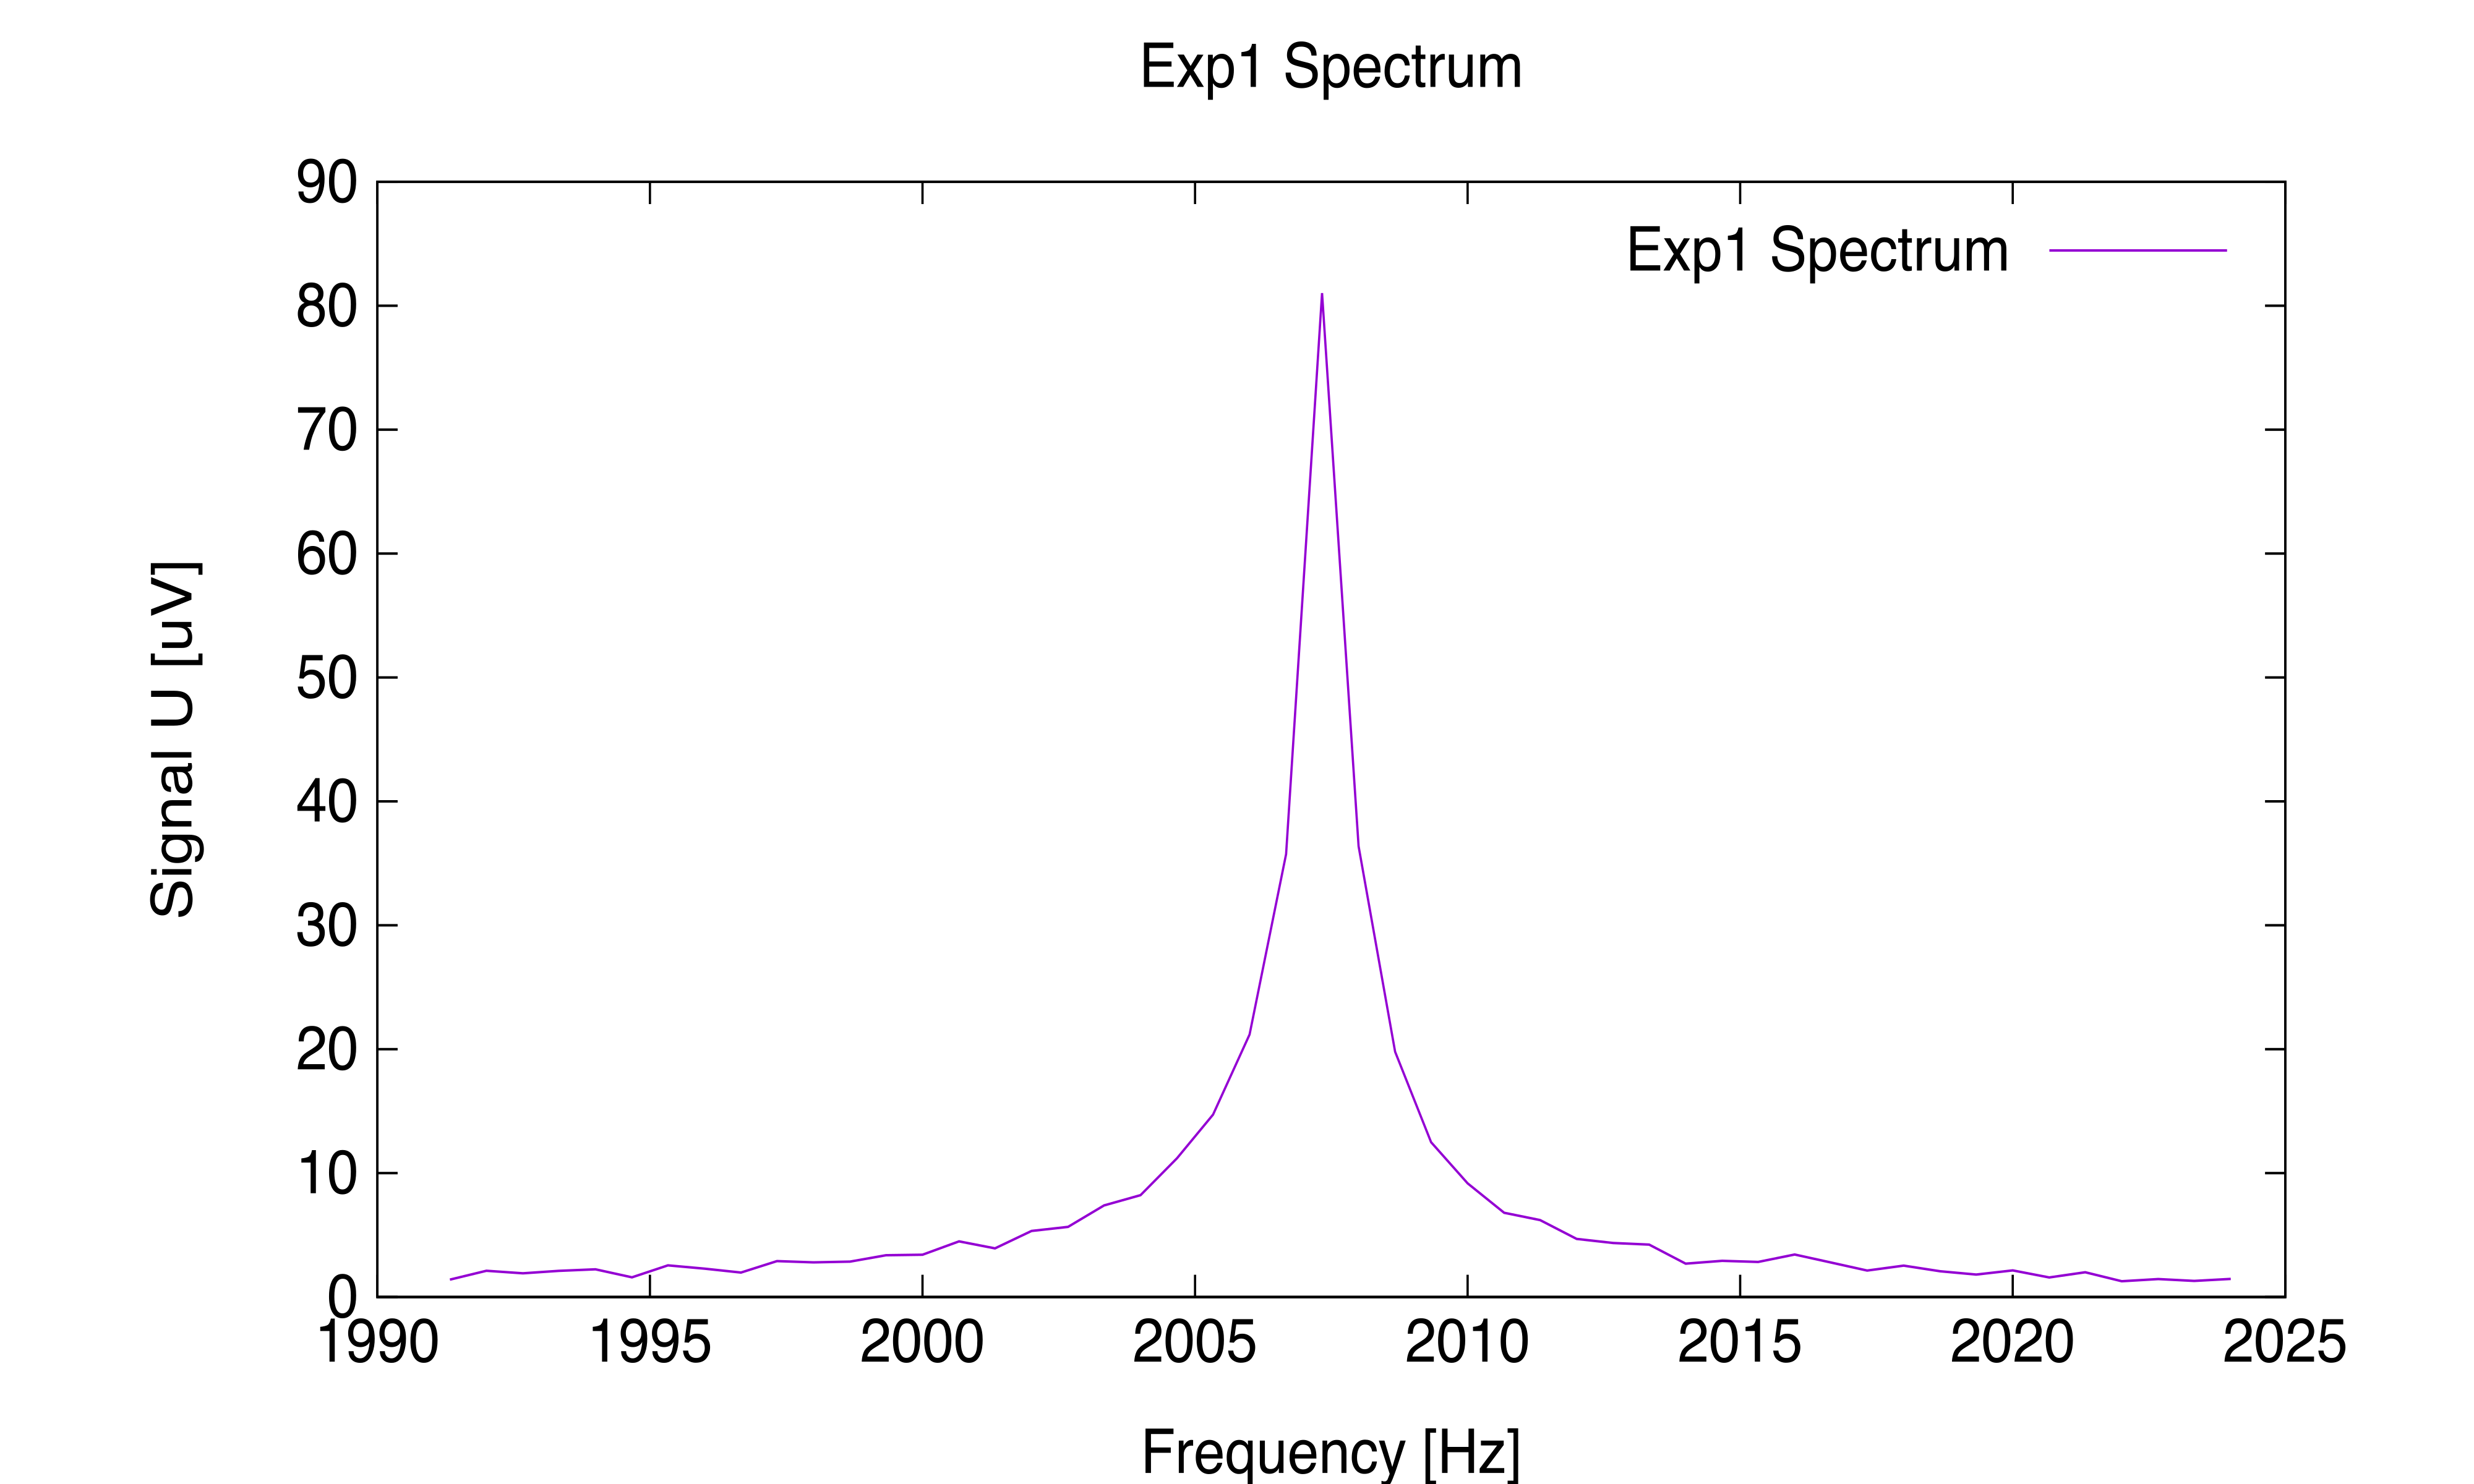
\includegraphics[width=6cm]{Bilddateien/2/Exp1_Spectrum.png}
            \caption{Spektrum des FIDs mit Larmorfrequenz $f_L = \SI{2007.33}{\hertz}$.}
            \label{fig:2:Spectrum-1}
        \end{subfigure}
        \
        \begin{subfigure}[b]{0.4\textwidth}
            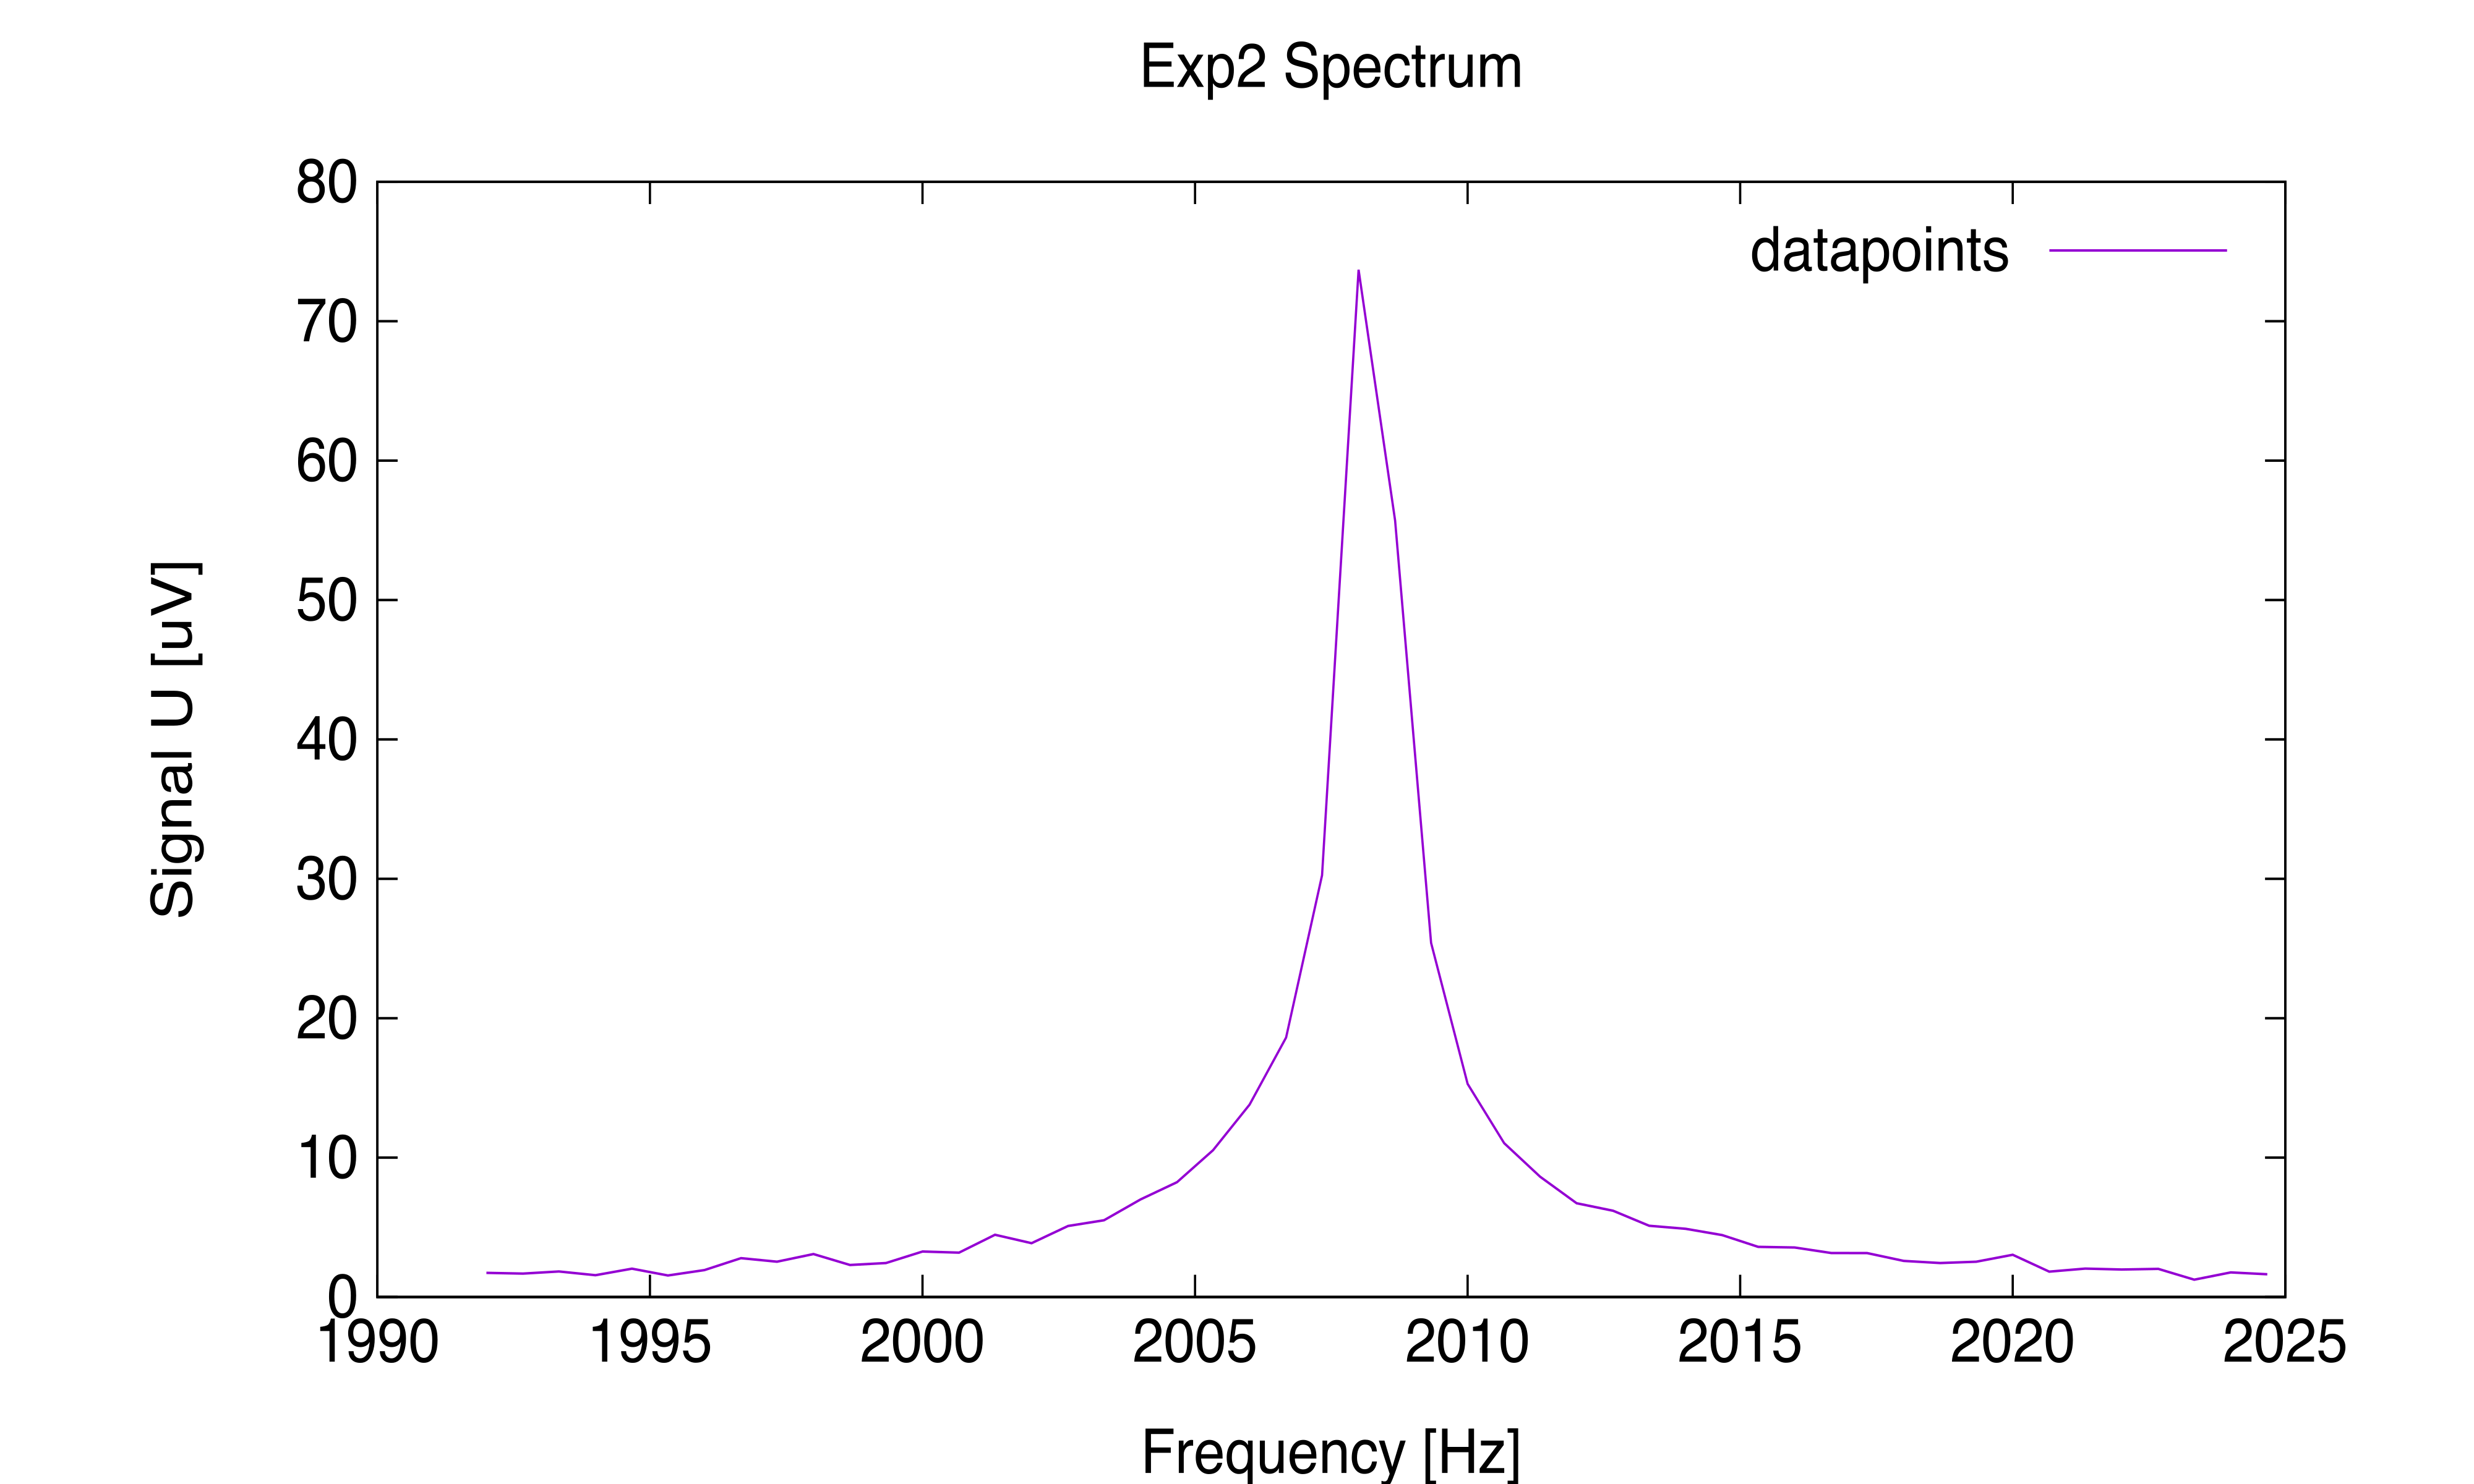
\includegraphics[width=6cm]{Bilddateien/2/Exp2_Spectrum.png}
            \caption{Spektrum des FIDs mit Larmorfrequenz $f_L = \SI{2000}{\hertz}$.}
            \label{fig:2:Spectrum-2}
        \end{subfigure}
        \caption{Spektren der FIDs mit den ermittelten Larmorfrequenzen.}
        \label{fig:2:Spectrum}
    \end{figure}
    Ein Blick auf die tatsächlichen Messdaten liefert uns die in Tabelle \ref{tab:2:Larmor_Freq} aufgeführten Werte. Die Unsicherheit der $U_{\textit{FID}}$ Spannung ist dabei durch die Standardabweichung der FID Werte gegeben.
    \begin{table}[H]
        \centering
        \begin{tabular}{c|l|l|r}
            \textbf{Durchgang} & $f_L$ in $\si{\hertz}$ & $U_{\textit{FID}}$ in $\si{\micro\volt}$ & $u(U_{\textit{FID}})$ in $\si{\micro\volt}$\\
            \hline
            $1$ & $2007.33$ & $81.02$ & $25.46$\\
            $2$ & $2000$ & $73.69$ & $26.01$ \\
            \hline 
            avg. & $2003.67$ & $77.36$ & $36.39$
        \end{tabular}
        \caption{Messwerte der Larmorfrequenz $f_L$ und die Unsicherheit der FID Amplutude $U_{\textit{FID}}$ zusammen mit dem bei $f_L$ gemessenen Signal in zwei Durchgängen.}
        \label{tab:2:Larmor_Freq}
    \end{table}
    An dieser Stelle macht es keinen Sinn, eine direkte Aussage über die Unsicherheit in $f_L$ zu tätigen, da diese gerätespezifisch aufgelöst wird und unter der Fouriertransformation mit der Signalunsicherheit des FIDs zusammenhängt. Eine Berechnung der Standardabweichung bei homogen verteilten Testwerten macht ebenfalls keinen Sinn. In den Graphen \ref{fig:2:Spectrum-1} und \ref{fig:2:Spectrum-2} sind die Peaks bei den ermittelten Larmorfrequenzen jedoch deutlich und scharf erkennbar.
    
\end{document}